\documentclass[12pt]{article}

\usepackage{graphicx}

\title{EECS 440 PA3 Writeup}
\author{Andrew Mason}

\begin{document}
\maketitle

\begin{enumerate}
    \item T-Tests for Voting, Volcanoes, and Spam\\
        \begin{tabular}{|r|c|c|}
          \hline
          Dataset & NBayes Accuracy & LogReg Accuracy \\ \hline
          Voting & 0.961 & 0.991 \\ \hline
          Volcanoes & 0.645 & 0.852 \\ \hline
          Spam & 0.704 & 0.706 \\ \hline
        \end{tabular}\\

        \begin{tabular}{|r|c|c|c|c|}
          \hline
          Dataset & F & V(F) & $\sigma$ & 95\% CI \\ \hline
          Voting & -0.030 & 0.00010545 & 0.0103 & (-0.0502, -0.0098)\\ \hline
          Volcanoes & -0.207 & 0.000159153 & 0.0126 & (-0.2317, -0.1823) \\ \hline
          Spam & -0.002 & 0.000005566 & 0.0024 & (-0.0067, 0.0027)\\ \hline
        \end{tabular}\\

        Since 0 is not in the 95\% CI for voting or volcanoes, logistic
        regression is actually superior for these datasets. Since 0 is in the
        95\% CI for spam, naive bayes and logistic regression have the same
        performance.
    \item Comparison with learning algorithms from previous assignments\\
        \begin{enumerate}
            \item Performance metrics\\
                For Voting, there was negligible improvement, but Voting
                had good performance on the previous assignments, anyways.
                For Volcanoes and Spam, logistic regression in particular
                saw tremendous improvement, boasting AUCs higher by at least
                0.2 for each dataset (0.9 for Volcanoes, 0.74 for Spam). Naive
                Bayes was not as remarkable, achieving AUCs (0.74, 0.54) much
                closer to that of the ANNs and decision trees.
            \item Runtime\\
                Both Naive Bayes and logistic regression were tremendously
                fast, with runtimes even for the largest dataset on the order
                of minutes. For comparison, the ANN was running on the order of
                hours (>= 20) for Spam. Adding in the parameter tuning did slow
                down the learning by a considerable amount (~1.5 hours for
                Spam), but this was bottlenecked by the computation of AUC for
                each parameter, as this was the performance metric I attempted
                to maximize in my parameter tuning.

                Another point here is that I got much better at numpy this time
                around, and was able to normalize my input for logistic
                regression in around 4 lines of numpy, with no iteration in
                Python, whereas to do the same in the ANN, I used nested Python
                loops and almost no numpy. This probably drastically affected
                the speed of training.
            \item Code complexity and implementation\\
                Both naive bayes and logistic regression were incredibly
                easy and straightforward to implement. Naive bayes is just
                counting, so with numpy there is nothing fancy to do there.
                Logistic regression is a little more complex, but since it is
                another gradient descent, having already implemented ANN, this
                was also very straightforward, and since I already had an idea
                of what I was doing, I was able to simplify things in my
                logistic regression implementation that I made unnecessarily
                complicated in my ANN implementation.
        \end{enumerate}
    \item Parameter tuning choices\\
        \begin{enumerate}
            \item m\\
                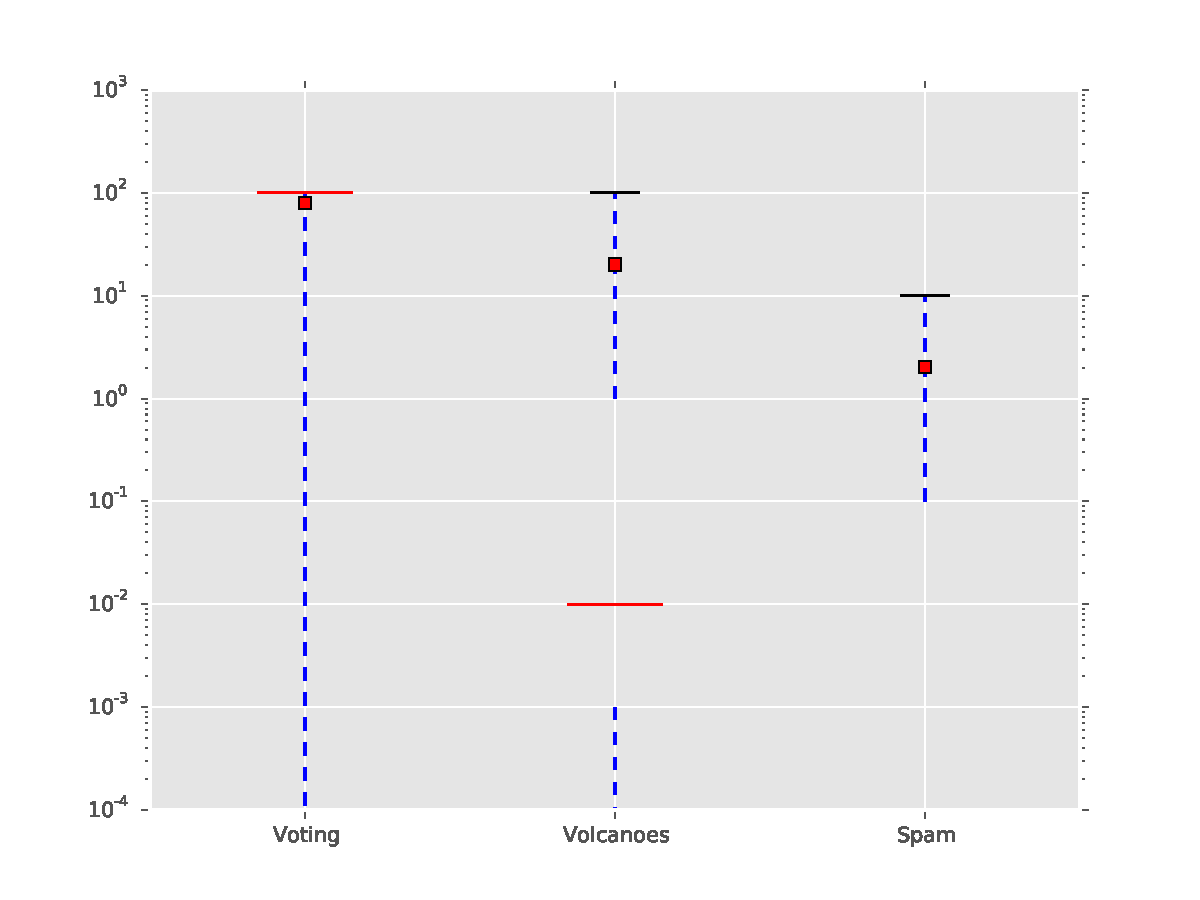
\includegraphics[width=\linewidth]{mchoices.pdf}
            \item $\lambda$\\
                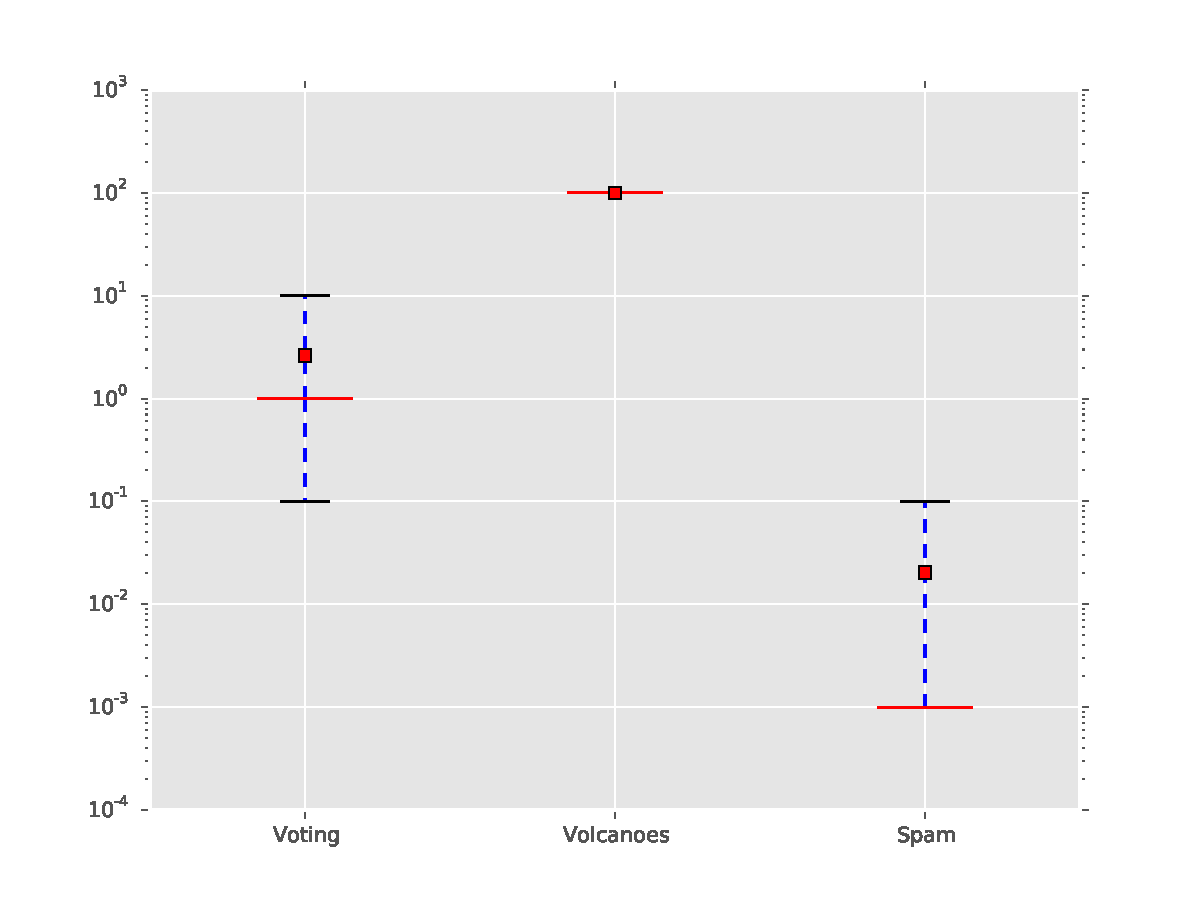
\includegraphics[width=\linewidth]{lambdachoices.pdf}
        \end{enumerate}

        Logistic regression did a much better job of ``settling in'' on a
        parameter choice (with Volcanoes having 100 chosen uniformly). This is
        most likely due to logistic regression being more tolerant to noise in
        the training samples. With minor adjustments in the counts from
        m-estimates, naive bayes can come up with widely varying predictions,
        so this would explain why naive bayes was less consistent (and saw
        less benefit - see part 4) in its choice of m.
    \item Tuning vs MLE\\
        \begin{enumerate}
            \item NBayes Tuned\\
            \begin{tabular}{|r|c|c|c|}
                \hline
                Metric & Voting & Volcanoes & Spam\\ \hline
                Accuracy & .961 & .645 & .704 \\ \hline
                Precision & .995 & .475 & .743 \\ \hline
                Recall & .918 & .799 & .806 \\ \hline
                AUC & .954 & .740 & .538 \\ \hline
            \end{tabular}\\
            \item NBayes MLE\\
            \begin{tabular}{|r|c|c|c|}
                \hline
                Metric & Voting & Volcanoes & Spam\\ \hline
                Accuracy & .984 & .658 & .705 \\ \hline
                Precision & .981 & .486 & .743 \\ \hline
                Recall & .985 & .751 & .806 \\ \hline
                AUC & .961 & .721 & .538 \\ \hline
            \end{tabular}\\
            \item LogReg Tuned\\
            \begin{tabular}{|r|c|c|c|}
                \hline
                Metric & Voting & Volcanoes & Spam\\ \hline
                Accuracy & .991 & .852 & .706 \\ \hline
                Precision & 1.00 & .840 & .728 \\ \hline
                Recall & .980 & .676 & .848 \\ \hline
                AUC & .995 & .900 & .742 \\ \hline
            \end{tabular}\\
            \item LogReg MLE\\
            \begin{tabular}{|r|c|c|c|}
                \hline
                Metric & Voting & Volcanoes & Spam\\ \hline
                Accuracy & .989 & .826 & .706 \\ \hline
                Precision & .995 & .747 & .728 \\ \hline
                Recall & .980 & .709 & .847 \\ \hline
                AUC & .996 & .882 & .742 \\ \hline
            \end{tabular}\\
        \end{enumerate}

        So, Nbayes did not have any remarkable improvment from the parameter
        tuning, but Logistic regression improved across nearly all datasets
        and metrics when using tuned parameters.
\end{enumerate}
\end{document}
